

\chapter{Aplikacja}
Aplikacja udostępnia prostą wizualizację oraz metody kontrolowania i podglądu stanu symulacji. Ten rozdział opisuje interfejs, obsługę i działanie aplikacji.

\section{Działanie aplikacji}
Po uruchomieniu użytkownik proszony jest o wybranie pliku \texttt{.json} z ustawieniami. Następnie tworzona jest instancja kontrolera osiołka i uruchamiane są zadania cykliczne: odświeżanie grafiki i obliczanie kolejnych tur symulacji. Program przyjmuje jeden opcjonalny argument wywołania: liczbę całkowitą określającą liczbę odświeżeń grafiki na sekundę. Wartość domyślna tego argumentu wynosi 20.

W momencie śmierci osiołka symulacja jest resetowana, ale licznik tur i kontroler zachowują swoje stany.

\clearpage

\section{Opis interfejsu}
\begin{figure}[H]
    \centering
    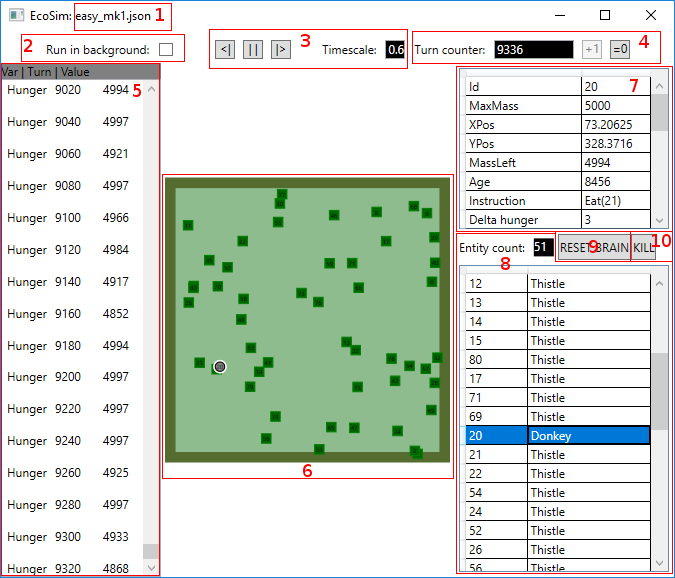
\includegraphics[scale=0.55]{Chapters/interface_annotated}
    \end{figure}
\begin{interface_descs}
    \item Nazwa wybranego pliku z ustawieniami.
    \item Checkbox pozwalający wyłączyć odświeżanie grafiki i obliczać kolejne tury symulacji tak szybko, jak jest to możliwe.
    \item Przyciski kontrolujące częstotliwość obliczania kolejnych tur symulacji.
    \item Licznik tur. Przycisk \textit{+1} pozwala obliczyć kolejną turę symulacji gdy \textbf{Timescale} jest równe 0. Przycisk \textit{=0} resetuje licznik tur.
    \item Log, w którym pojawiają się wiadomości tworzone przez symulację. W przykładzie jest to bieżąca tura i stan żołądka osiołka wypisywane co 20 tur.
    \item Plansza reprezentująca stan symulacji.
    \item Szczegóły obecnie wybranego bytu. Byt można wybrać klikając go na planszy lub na liście bytów.
    \item Lista bytów znajdujących się na planszy.
    \item Przycisk pozwalający wywołać metodę \textit{Reset()} na kontrolerze osiołka, która ponownie inicjalizuje jego stan wartościami początkowymi.
    \item Przycisk pozwalający natychmiastowo zabić obecną instancję osiołka.
\end{interface_descs}

\section{Ustawienia}
Symulacja oraz kontroler są parametryzowane plikiem \texttt{.json}. Poniżej przedstawiam przykładowy plik z ustawieniami oraz ich opisami:
\begin{figure}[h]
\label{fig:example_settings}
\begin{lstlisting}[language=json_comment]
{
"Brain": "Mark1", //"Mark1" lub "Mark0", wybiera rodzaj kontrolera

"LogDeaths" : false, //wartość true sprawia, że po każdej śmierci osiołka zalogowana zostanie tura jego urodzin i wiek w momencie zgonu

"LogHungerEvery": 20, //loguje stan żołądka osiołka co każde LogHungerEvery tur. Wartość 0 wyłącza tę opcję.

"InitialPlantCount": 20, //liczba roślin pojawiająca się na początku symulacji

"MaxPlantCount": 50, //maksymalna liczba roślin na planszy

"NewPlantFrequency": 5, //liczba tur między pojawieniami się nowych roślin

"MinPlantMass": 100, //dolna granica przedziału, z którego losowana jest maksymalna masa rośliny
"MaxPlantMass": 500, //górna granica w/w przedziału

"MinGrowthRate": 30, //dolna granica przedziału, z którego losowany jest parametr RegrowthRate rośliny
"MaxGrowthRate": 50, //górna granica w/w przedziału

// opisane w rozdz. 2 pracy:
"MovementSpeed": 20,         
"InteractionDistance": 22,         
"BiteSize": 100,         
"StomachCapacity": 5000,        
"SightRange": 88, 
"PassiveWork": 3,
"MovementWork": 5,

// opisane w rozdz. 4 pracy:
"BrainBaseActionScore": 0.0022,
"BrainDiscount": 0.6,        
"BrainLearningRate": 0.148,        
"BrainLearningRateDamping": 0.99999,         
"BrainBaseActionScoreDamping" : 0.99952,         
"BrainProbabilityExponent": 1.6 
}
\end{lstlisting}
\end{figure}
